\documentclass[11pt]{article}
\usepackage[letterpaper,textwidth=5.8in,textheight=8.9in]{geometry}
\usepackage{amsmath,amssymb,graphicx,booktabs,array,tabularx,multirow}
\usepackage[numbers,sort&compress]{natbib}
\usepackage[hidelinks]{hyperref}
\usepackage{microtype}
\usepackage{xcolor}
\usepackage[font=small,labelfont=bf]{caption}
\usepackage[section]{placeins}  % keep each section's floats inside the section
\renewcommand{\topfraction}{0.92}
\renewcommand{\bottomfraction}{0.8}
\renewcommand{\textfraction}{0.06}
\renewcommand{\floatpagefraction}{0.8}
\setcounter{topnumber}{3}
\setcounter{bottomnumber}{2}
\setcounter{totalnumber}{4}
\usepackage{tikz}
\usetikzlibrary{positioning,fit,backgrounds,arrows.meta,calc}
\setlength{\emergencystretch}{2em}
\newcommand{\figpath}{../figures}
\newcommand{\code}[1]{\texttt{#1}}
\newcolumntype{L}{>{\raggedright\arraybackslash}X}

% one colour per role, shared with the plots
\definecolor{wam}{HTML}{D55E00}
\definecolor{vla}{HTML}{0072B2}
\definecolor{ink}{HTML}{333333}

\tikzset{
  box/.style={draw=ink, rounded corners=2pt, align=center, inner sep=2.5pt, minimum height=6mm, fill=white, font=\footnotesize},
  io/.style={align=center, inner sep=1pt, font=\footnotesize},
  lat/.style={draw=ink, circle, align=center, inner sep=0.5pt, minimum size=8.5mm, fill=gray!8, font=\footnotesize},
  ours/.style={box, draw=wam, fill=wam!10, thick},
  flow/.style={-{Stealth[length=1.7mm]}, ink},
  aflow/.style={-{Stealth[length=1.7mm]}, wam, dashed},
  lbl/.style={font=\scriptsize, text=ink!80, align=center},
  opt/.style={draw=ink!40, rounded corners=2pt, align=center, inner sep=2pt, text width=2.55cm, minimum height=5.5mm, fill=white, font=\scriptsize},
  pick/.style={opt, draw=wam, fill=wam!12, thick},
  head/.style={align=center, font=\footnotesize\bfseries, text width=2.7cm},
}

\title{pico-WAM: Design and Evaluation of a\\Compact World Action Model}
\author{Keivalya Pandya\\Northeastern University}
\date{}

\begin{document}
\maketitle

\begin{abstract}
World action models combine action generation with prediction of future observations or states. Their implementations differ in the prediction target, model architecture, and use of predictions during control. We present pico-WAM, a 0.75M-parameter implementation for studying these choices in a navigation environment with known dynamics. A shared representation supports a policy, an action-conditioned transition model, and state and image readouts. We compare this design with eight open-source systems and evaluate prediction accuracy, policy performance, and computational cost. Across three runs, pico-WAM predicts states 15 steps ahead with approximately $80\times$ lower normalized error than persistence, although its image predictions are worse than copying the current frame. Training on expert-only trajectories gives lower long-horizon factual error but approximately $15\times$ higher error under alternative actions than training with random-action bursts. With pixel inputs, the full objective improves policy success from 36\% to 80\%. A separate five-run pilot shows that current-state supervision contributes more of the measured gain than future-state prediction. Finally, removing image decoding reduces optimizer-step time by about 90\% in a single-thread CPU benchmark. These results identify useful controls for evaluating small world action models and separate the effects of prediction targets, training data, and auxiliary supervision.

\end{abstract}

% =====================================================================
\section{Introduction}

A vision-language-action (VLA) policy maps observations and instructions to actions. An action-conditioned world model predicts how the environment changes under a specified action. World action models (WAMs) combine these functions through joint prediction, inverse dynamics, or planning \citep{lu2026survey,shen2026survey}. We study joint training: a policy and forward model share a representation, but only the policy is used during control (Figure~\ref{fig:paradigms}).

\begin{figure}[!htbp]
\centering
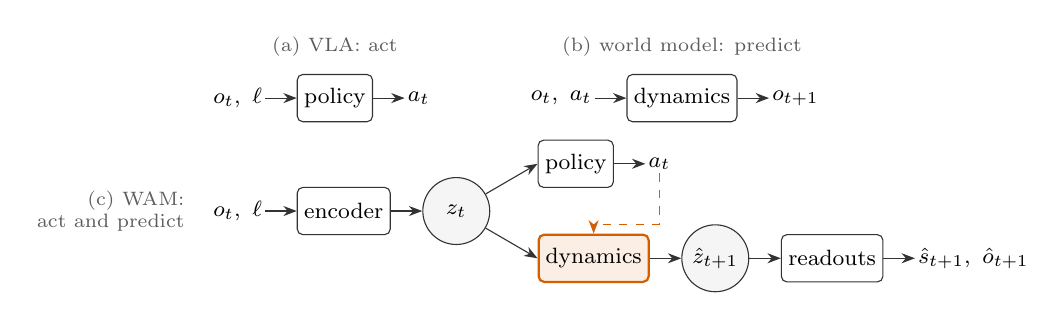
\begin{tikzpicture}[node distance=2.5mm and 4mm]
  % (a) VLA
  \node[io] (o1) {$o_t,\ \ell$};
  \node[box, right=of o1] (p1) {policy};
  \node[io, right=of p1] (a1) {$a_t$};
  \draw[flow] (o1) -- (p1); \draw[flow] (p1) -- (a1);
  \node[lbl, above=1mm of p1] {(a) VLA: act};
  % (b) world model
  \node[io, right=12mm of a1] (o2) {$o_t,\ a_t$};
  \node[box, right=of o2] (f2) {dynamics};
  \node[io, right=of f2] (s2) {$o_{t+1}$};
  \draw[flow] (o2) -- (f2); \draw[flow] (f2) -- (s2);
  \node[lbl, above=1mm of f2] {(b) world model: predict};
  % (c) WAM
  \node[io, below=11mm of o1] (o3) {$o_t,\ \ell$};
  \node[box, right=of o3] (e3) {encoder};
  \node[lat, right=of e3] (z3) {$z_t$};
  \node[box, right=6mm of z3, yshift=6mm] (p3) {policy};
  \node[io, right=of p3] (a3) {$a_t$};
  \node[ours, right=6mm of z3, yshift=-6mm] (f3) {dynamics};
  \node[lat, right=of f3] (z31) {$\hat z_{t+1}$};
  \node[box, right=of z31] (r3) {readouts};
  \node[io, right=of r3] (y3) {$\hat s_{t+1},\ \hat o_{t+1}$};
  \draw[flow] (o3) -- (e3); \draw[flow] (e3) -- (z3);
  \draw[flow] (z3) -- (p3.west); \draw[flow] (z3) -- (f3.west);
  \draw[flow] (p3) -- (a3); \draw[flow] (f3) -- (z31); \draw[flow] (z31) -- (r3); \draw[flow] (r3) -- (y3);
  \draw[aflow] (a3.south) |- ($(f3.north)+(0,1.2mm)$) -- (f3.north);
  \node[lbl, left=2mm of o3, anchor=east, align=right] {(c) WAM:\\act and predict};
\end{tikzpicture}
\caption{\textbf{Policy prediction, forward prediction, and joint training.} (a) A policy maps observation $o_t$ and instruction $\ell$ to action $a_t$. (b) An action-conditioned forward model predicts a future observation. (c) In pico-WAM, a policy and transition model share latent state $z_t$. The transition model accepts a specified action, and readouts convert its predicted latent into a physical state and image. Repeated transitions generate an open-loop rollout. The deployed policy does not use this rollout for action selection.}
\label{fig:paradigms}
\end{figure}

Several recent WAMs use billion-parameter video backbones \citep{liao2025genie,kim2026cosmospolicy,li2026lingbotva}, making controlled comparisons expensive. Tutorials describe their design choices \citep{zhang2026tutorial}, and minimal video-prediction implementations simplify some components \citep{huang2026nano}. A small model containing both a policy and a predictor allows their interaction to be tested directly.

We present pico-WAM, a 747,739-parameter model with image, instruction, and state encoders, an action head, latent dynamics, and state and image decoders. Its point-mass environment permits exact simulation of alternative actions. We use this setting to ask whether prediction along recorded trajectories generalizes to other actions, whether auxiliary prediction improves the policy, and which components account for its cost.

The paper compares eight open-source systems, evaluates data coverage and training objectives in pico-WAM, and profiles its parameters and runtime. The architecture uses established components; the contribution is an implementation and empirical study of their behavior.

% =====================================================================
\section{Prediction and control in existing systems}
\label{sec:design}

We compare systems along four dimensions: the prediction target, the relation between actions and predictions, the model architecture, and the use of predicted futures (Figure~\ref{fig:design}). These dimensions describe design choices rather than mutually exclusive model classes. For example, joint training can include an action-conditioned forward model, and a video model can serve both as a predictor and as a source of synthetic data. Table~\ref{tab:wams} includes such related systems alongside joint policy--prediction models.

\begin{figure}[!htbp]
\centering
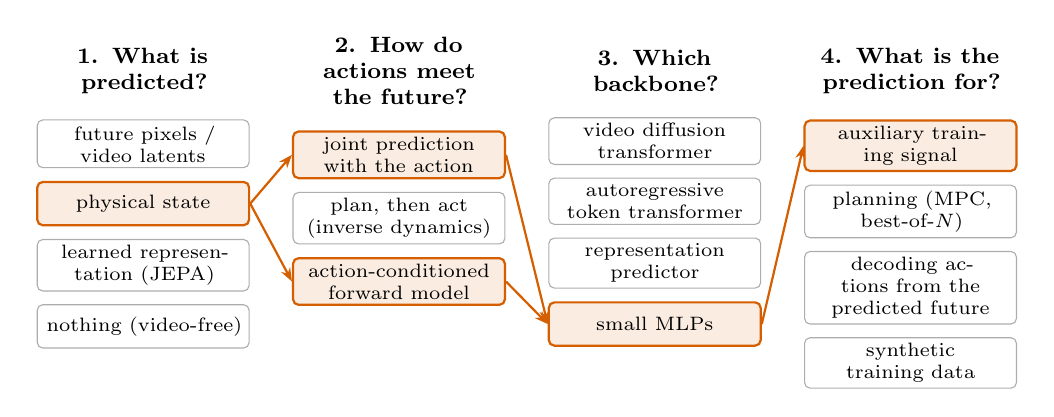
\begin{tikzpicture}[node distance=1.6mm and 3mm]
  \node[head] (h1) {1. What is predicted?};
  \node[head, right=of h1] (h2) {2. How do actions meet the future?};
  \node[head, right=of h2] (h3) {3. Which backbone?};
  \node[head, right=of h3] (h4) {4. What is the prediction for?};
  % column 1
  \node[opt, below=2mm of h1] (c11) {future pixels / video latents};
  \node[pick, below=of c11] (c12) {physical state};
  \node[opt, below=of c12] (c13) {learned representation (JEPA)};
  \node[opt, below=of c13] (c14) {nothing (video-free)};
  % column 2
  \node[pick, below=2mm of h2] (c21) {joint prediction with the action};
  \node[opt, below=of c21] (c22) {plan, then act (inverse dynamics)};
  \node[pick, below=of c22] (c23) {action-conditioned forward model};
  % column 3
  \node[opt, below=2mm of h3] (c31) {video diffusion transformer};
  \node[opt, below=of c31] (c32) {autoregressive token transformer};
  \node[opt, below=of c32] (c33) {representation predictor};
  \node[pick, below=of c33] (c34) {small MLPs};
  % column 4
  \node[pick, below=2mm of h4] (c41) {auxiliary training signal};
  \node[opt, below=of c41] (c42) {planning (MPC, best-of-$N$)};
  \node[opt, below=of c42] (c43) {decoding actions from the predicted future};
  \node[opt, below=of c43] (c44) {synthetic training data};
  \draw[wam, thick, -{Stealth[length=1.7mm]}] (c12.east) -- (c21.west);
  \draw[wam, thick, -{Stealth[length=1.7mm]}] (c12.east) -- (c23.west);
  \draw[wam, thick, -{Stealth[length=1.7mm]}] (c21.east) -- (c34.west);
  \draw[wam, thick, -{Stealth[length=1.7mm]}] (c23.east) -- (c34.west);
  \draw[wam, thick, -{Stealth[length=1.7mm]}] (c34.east) -- (c41.west);
\end{tikzpicture}
\caption{\textbf{Design choices in predictive control systems.} The columns distinguish prediction target, action modeling, architecture, and use of predictions. Orange marks pico-WAM's main configuration: state prediction, joint policy--dynamics training, an action-conditioned MLP transition, and auxiliary supervision. Image decoding is optional. Choices can overlap; for example, a jointly trained model can also support forward prediction under supplied actions. Table~\ref{tab:wams} compares the main configurations of eight related systems.}
\label{fig:design}
\end{figure}

\begin{table}[!htbp]
\centering\footnotesize
\begin{tabularx}{\linewidth}{>{\hsize=0.72\hsize}L >{\hsize=0.98\hsize}L >{\hsize=1.12\hsize}L >{\hsize=0.98\hsize}L >{\hsize=1.2\hsize}L}
\toprule
System & Predicts & Backbone & Action decoding & Future used for \\
\midrule
GR-1 \citep{wu2023gr1} & future frames (image patches) & GPT-style causal transformer, video-pretrained on Ego4D clips & linear head on an \texttt{[ACT]} token & training signal \\
UWM \citep{zhu2025uwm} & video and actions & one diffusion transformer, independent timesteps per modality & action diffusion & policy, forward or inverse dynamics, video generation \\
WorldVLA \citep{cen2025worldvla} & next frame (VQ tokens) & autoregressive multimodal LLM (Chameleon init.) & discrete action tokens & training signal \\
Genie Envisioner \citep{liao2025genie} & video chunks & video diffusion transformer (2B) & flow-matching action module on video latents & action decoding; neural simulator \\
Cosmos Policy \citep{kim2026cosmospolicy} & future states and values as latent frames & Cosmos-Predict2 video diffusion (2B) & actions injected as latent frames & best-of-$N$ planning \\
V-JEPA 2-AC \citep{assran2025vjepa2} & future representations & frozen V-JEPA 2 encoder + 300M action-conditioned predictor & none: actions come from the planner & CEM model-predictive control \\
DreamGen \citep{jang2025dreamgen} & robot videos & fine-tuned video generation model & inverse dynamics or latent actions label the videos & synthetic training data \\
LingBot-VA \citep{li2026lingbotva} & video latents, autoregressively & dual-stream diffusion transformer (5.3B), KV cache & inverse dynamics from the predicted future & action decoding; memory \\
\midrule
\textbf{pico-WAM} (ours) & physical state, pixels, latents & 3-layer CNN + GRU + MLPs (0.75M) & MLP, diffusion or flow head & training signal; analysis \\
\bottomrule
\end{tabularx}
\caption{\textbf{Comparison of eight open-source predictive robot-learning systems and pico-WAM.} Entries describe the main configuration reported in each paper. The table includes joint policy models, forward models used by planners, and video generators used to create training data. Their prediction targets and deployment roles differ, so model size alone is not a comparison of capability.}
\label{tab:wams}
\end{table}

These deployment roles require different evaluations. Auxiliary prediction should be judged by its effect on the deployed policy; planning additionally requires accurate comparisons between candidate actions. Synthetic-data methods must be evaluated through policies trained on their generated data. pico-WAM studies the first setting and tests its forward model separately.

GR-1's future-frame objective \citep{wu2023gr1}, Cosmos Policy's action selection \citep{kim2026cosmospolicy}, and V-JEPA 2-AC's representation-space planning \citep{assran2025vjepa2} motivate our tests of prediction horizon, action coverage, and decoding cost. The toy setting makes these choices inexpensive to examine, but cannot establish that the same mechanisms explain results in large robot models.

% =====================================================================
\section{Model and experimental setup}
\label{sec:build}

\begin{figure}[!htbp]
\centering
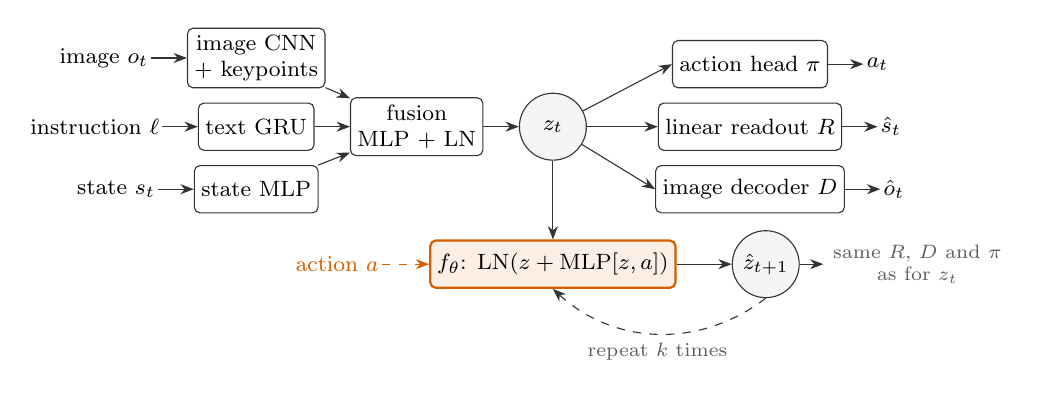
\begin{tikzpicture}[node distance=2.5mm and 4.5mm]
  \node[box] (te) {text GRU};
  \node[box, above=1.8mm of te] (ie) {image CNN\\+ keypoints};
  \node[box, below=1.8mm of te] (se) {state MLP};
  \node[io, left=of ie] (img) {image $o_t$};
  \node[io, left=of te] (txt) {instruction $\ell$};
  \node[io, left=of se] (st) {state $s_t$};
  \node[box, right=of te] (fu) {fusion\\MLP + LN};
  \node[lat, right=of fu] (z) {$z_t$};
  \foreach \u/\v in {img/ie, txt/te, st/se, ie/fu, te/fu, se/fu, fu/z} \draw[flow] (\u) -- (\v);
  \node[box, right=9mm of z] (ro) {linear readout $R$};
  \node[box, above=1.8mm of ro] (pol) {action head $\pi$};
  \node[box, below=1.8mm of ro] (dec) {image decoder $D$};
  \foreach \v in {pol, ro, dec} \draw[flow] (z) -- (\v.west);
  \node[io, right=of pol] (a) {$a_t$};
  \node[io, right=of ro] (sh) {$\hat s_t$};
  \node[io, right=of dec] (ih) {$\hat o_t$};
  \draw[flow] (pol) -- (a); \draw[flow] (ro) -- (sh); \draw[flow] (dec) -- (ih);
  \node[ours, below=10mm of z] (dyn) {$f_\theta$: $\mathrm{LN}(z + \mathrm{MLP}[z, a])$};
  \node[io, left=6mm of dyn, text=wam] (act) {action $a$};
  \node[lat, right=7mm of dyn] (z1) {$\hat z_{t+1}$};
  \draw[flow] (z) -- (dyn); \draw[aflow] (act) -- (dyn); \draw[flow] (dyn) -- (z1);
  \node[lbl, right=3mm of z1] (z1out) {same $R$, $D$ and $\pi$\\as for $z_t$};
  \draw[flow] (z1) -- (z1out);
  \draw[flow, dashed] (z1.south) to[bend left=40] node[lbl, below] {repeat $k$ times} (dyn.south);
\end{tikzpicture}
\caption{\textbf{pico-WAM architecture.} Image, instruction, and state encoders produce features that are fused into $z_t$. The action head, linear state readout $R$, and image decoder $D$ use this representation. The residual transition model $f_\theta$ predicts the next latent from $(z_t,a_t)$; the same readouts decode subsequent latents. Layer normalization controls latent scale but does not ensure that predicted and encoded latents have identical distributions. Figure~\ref{fig:efficiency} reports parameter counts.}
\label{fig:arch}
\end{figure}

\paragraph{Architecture.} The observation comprises a $64\times64$ RGB image $o_t$, an instruction $\ell$, and, when available, a six-dimensional state $s_t$. A three-layer CNN, a text GRU, and a state MLP encode these inputs. The image encoder combines 16 spatial-softmax keypoints with pooled image features. A fusion MLP followed by layer normalization produces $z_t\in\mathbb R^{128}$ (Figure~\ref{fig:arch}).

The policy maps $z_t$ to a two-dimensional action. The implementation supports MLP, diffusion, and flow heads; the reported control experiments use the MLP head. The transition model is a residual MLP, $f_\theta(z,a)=\operatorname{LN}(z+\operatorname{MLP}[z,a])$. Starting from $\hat z_t=z_t$, it predicts successive latents through $\hat z_{t+k+1}=f_\theta(\hat z_{t+k},a_{t+k})$. A linear readout $R$ predicts the normalized physical state, and a decoder $D$ predicts an image residual relative to the training-set mean image. Both readouts apply to encoded and predicted latents. Because $R$ is trained with state labels, its accuracy measures supervised state reconstruction, not independently discovered physical structure.

\paragraph{Training objective.} Each sample is a window of $H$ transitions from one episode. The model encodes the initial observation and predicts the next $H$ latents using the recorded actions (Figure~\ref{fig:train}). Training minimizes
\begin{equation}
\mathcal L=\mathcal L_{\mathrm{act}}+w_s\mathcal L_{\mathrm{state}}
+w_i\mathcal L_{\mathrm{image}}+w_z\mathcal L_{\mathrm{latent}}.
\label{eq:loss}
\end{equation}
The state loss adds current-state reconstruction MSE to mean future-state MSE across the $H$ predictions; the image loss has the same form. The latent loss averages MSE between predicted latents and stop-gradient encodings of the corresponding future observations. All MSE terms average over output coordinates. State targets use training-set means and standard deviations. The default weights are $w_s=0.5$ and $w_i=w_z=1$, with $H=5$.

The action loss is evaluated only on expert-labeled transitions. Removing the auxiliary objectives gives the behavioral-cloning comparator, labeled VLA in the figures. It uses the same encoder design and is trained from scratch. At deployment, both policies encode the current observation and emit an action; neither uses imagined states to select that action.

\begin{figure}[!htbp]
\centering
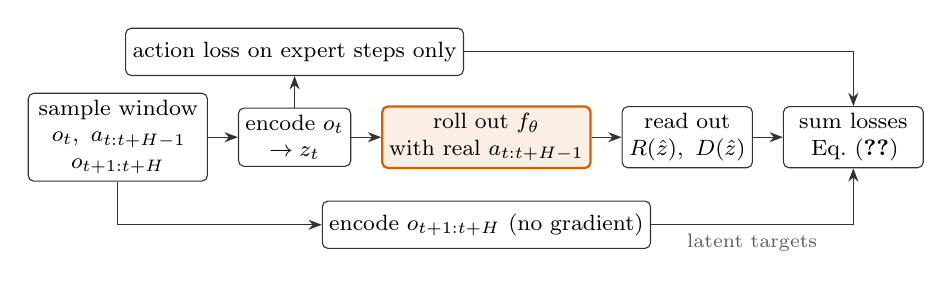
\begin{tikzpicture}[node distance=2.5mm and 3.8mm]
  \node[box, text width=2.1cm] (win) {sample window\\$o_t,\ a_{t:t+H-1}$\\$o_{t+1:t+H}$};
  \node[box, right=of win] (enc) {encode $o_t$\\$\rightarrow z_t$};
  \node[ours, right=of enc] (roll) {roll out $f_\theta$\\with real $a_{t:t+H-1}$};
  \node[box, right=of roll] (read) {read out\\$R(\hat z),\ D(\hat z)$};
  \node[box, right=of read, text width=1.6cm] (loss) {sum losses\\Eq.~\eqref{eq:loss}};
  \draw[flow] (win) -- (enc); \draw[flow] (enc) -- (roll); \draw[flow] (roll) -- (read); \draw[flow] (read) -- (loss);
  \node[box, below=4mm of roll] (tgt) {encode $o_{t+1:t+H}$ (no gradient)};
  \draw[flow] (win.south) |- (tgt.west);
  \draw[flow] (tgt.east) -| node[lbl, pos=0.25, below] {latent targets} (loss.south);
  \node[box, above=4mm of enc] (pol) {action loss on expert steps only};
  \draw[flow] (enc.north) -- (pol.south);
  \draw[flow] (pol.east) -| (loss.north);
\end{tikzpicture}
\caption{\textbf{Training on a window of $H$ transitions.} The initial observation is encoded with gradients, and the transition model is rolled forward using recorded actions. State and image readouts are trained against current and future targets. Future observations are encoded to form stop-gradient targets for latent consistency; they are not inputs to the rollout. The action loss uses only expert-labeled steps, whereas prediction losses use all sampled transitions.}
\label{fig:train}
\end{figure}

\paragraph{Environment and data.} The agent moves toward one of two colored goals selected by the instruction (Figure~\ref{fig:toy}). Position $p_t$ lies in the unit square, action $a_t\in[-1,1]^2$ applies a force, and physical velocity follows
\[
v_{t+1}=0.8v_t+0.01a_t,\qquad
p_{t+1}=\operatorname{clip}(p_t+v_{t+1},0,1).
\]
The observed state is $(p_t,v_t/0.05,g)$, where $g$ is the selected goal position. Success requires distance to $g$ below 0.05 and normalized speed below 0.2. A proportional--derivative controller supplies expert actions. When no random burst is active, the collector starts one with probability 0.3; its duration is sampled uniformly from one to three steps. Each burst action is sampled uniformly from $[-1,1]^2$. Thus 0.3 is the burst-start probability, not the fraction of random transitions.

In the state-input condition, the selected goal coordinates already identify the target, so the policy need not use language to select it. In the pixel-input condition, the state-encoder output is set to zero, but the WAM still receives state-prediction targets during training. Velocity is not rendered: one image can correspond to different velocities. We therefore distinguish pixel inputs from training without state supervision.

\begin{figure}[!htbp]
\centering
\includegraphics{\figpath/fig-toy-world.pdf}
\caption{\textbf{Navigation environment and data collection.} (a) Actual frames from an expert episode. The red agent must reach the instructed goal and slow down; the other colored square is a distractor. Images show positions but not velocity. (b) Actions from a collection episode, with random-action bursts shaded. When no burst is active, one starts with probability 0.3 and lasts one to three steps. These transitions contribute to prediction losses but are excluded from action regression.}
\label{fig:toy}
\end{figure}

\paragraph{Evaluation protocol.} Unless stated otherwise, each configuration uses three independent data, split, and initialization seeds, 400 collected episodes, a 90/10 episode split, and 15 training epochs. Closed-loop evaluation uses 100 unseen episodes per run. Prediction is evaluated on held-out episodes by encoding each valid starting observation once and rolling forward without observing later frames. Factual evaluation uses recorded actions. Counterfactual evaluation samples eight random action sequences at starts spaced five steps apart and compares each prediction with the simulator.

State error is mean squared error after dividing each coordinate's residual by its training-set standard deviation. Factual error averages all six state coordinates; counterfactual error averages only position and velocity. Image error is pixel MSE on RGB values scaled to $[0,1]$. Factual persistence repeats the initial state or image. The counterfactual reference instead runs the true simulator with zero actions from the same initial state.

The main study reports population standard deviations over three runs; the five-run supervision pilot reports sample standard deviations. These are measures of run-to-run variation, not confidence intervals. Overlapping prediction windows are correlated. Exploration conditions also change state distributions and normalization statistics, so their errors describe the resulting datasets rather than an isolated effect of action diversity.

% =====================================================================
\section{Experimental results}
\label{sec:lessons}

We first evaluate the forward model, then examine whether auxiliary prediction improves the policy. Table~\ref{tab:lessons} summarizes the main comparisons. It also records decoder and diffusion-schedule changes made during development; those observations are distinguished from the repeated experimental comparisons.

\begin{table}[!htbp]
\centering\footnotesize
\begin{tabularx}{\linewidth}{>{\hsize=0.7\hsize}L >{\hsize=1.0\hsize}L >{\hsize=1.5\hsize}L >{\hsize=0.8\hsize}L}
\toprule
Component & Comparison & Observation & Interpretation \\
\midrule
Training data & expert only vs.\ burst-start probability 0.3 & counterfactual error at $k{=}10$ falls from $0.112$ to $0.0072$, even though factual error is lower with expert-only data (Fig.~\ref{fig:coverage}) & lower counterfactual error \\
Imagination horizon $H$ & 1, 5, 10 steps & 10-step counterfactual error $0.0139$, $0.0072$, $0.0057$; one-step error $0.0019$, $0.0019$, $0.0030$ & short-/long-horizon trade-off \\
Latent consistency & on vs.\ off & 15-step error $0.0071\pm0.0004$ vs.\ $0.0096\pm0.0024$; one-step error slightly better without it & lower long-horizon error and spread \\
Image loss & on vs.\ off (state input) & 15-step state error $0.0071$ vs.\ $0.0074$ & similar observed means \\
Decoder output & sigmoid vs.\ residual on the mean image & sigmoid training stalled; the residual decoder learns, but remains worse than frame copying (Fig.~\ref{fig:imagine}c) & limited image fidelity \\
Visual representation & keypoints with vs.\ without state input & with state input the keypoints barely move; without it they track the agent ($R^2 \ge 0.998$) (Fig.~\ref{fig:keypoints}) & stronger localization without state input \\
Diffusion head & linear schedule ($\bar\alpha_T \approx 0.92$) vs.\ cosine ($\bar\alpha_T \approx 10^{-5}$) & the linear schedule never reaches noise, yet sampling starts from noise; fixed with a cosine schedule and the DDPM posterior & noise-schedule correction \\
Auxiliary supervision & BC, + current state, + future state (pixel input) & success $17.0\%$, $28.4\%$, $33.6\%$; current-state supervision gives the larger increment (Fig.~\ref{fig:policy}c) & future prediction adds 5.2 points \\
Few demonstrations & 25 to 400 episodes & WAM trails VLA at 25 episodes ($87\%$ vs.\ $99.7\%$); matched updates close most of the gap & sensitive to update budget \\
\bottomrule
\end{tabularx}
\caption{\textbf{Experimental comparisons and implementation observations.} State errors are normalized MSE, and policy success is measured on 100 unseen episodes per run. Main comparisons use three runs; the supervision pilot uses five. Decoder and diffusion-schedule rows describe development observations, not repeated ablations. Factual error averages six state coordinates; counterfactual error averages position and velocity only. Similar means do not establish equivalence.}
\label{tab:lessons}
\end{table}

\paragraph{State and image prediction.} At horizon 15, factual state NMSE is $0.0071\pm0.0004$, compared with $0.5824$ for persistence. At horizon 10, counterfactual error is $0.0072$, compared with $0.388$ for the zero-action simulator reference (Figure~\ref{fig:imagine}). The model therefore predicts motion substantially better than these references. The comparison does not establish an advantage over a fitted state-space model.

Image prediction is less successful. Pixel MSE exceeds frame copying at every evaluated horizon, despite accurate state readouts. In the episode shown in Figure~\ref{fig:strip}, the decoder retains the agent and selected goal but fails to reconstruct the distractor. This example illustrates a reconstruction failure; it does not establish why the distractor is lost. The large static background also makes copying a strong pixel baseline.

\begin{figure}[!htbp]
\centering
\includegraphics{\figpath/fig-imagination-quality.pdf}
\caption{\textbf{Prediction error versus rollout horizon.} (a) Factual normalized state MSE compared with persistence. (b) Counterfactual normalized MSE under random actions, compared with a true-simulator rollout that applies zero actions. (c) Pixel MSE compared with repeating the initial frame. Lines show means and bands population standard deviations across three runs, each with 40 held-out episodes. State prediction improves on these references; image prediction does not.}
\label{fig:imagine}
\end{figure}

\begin{figure}[!htbp]
\centering
\includegraphics{\figpath/fig-episode-strip.pdf}
\caption{\textbf{Observed and decoded frames from one held-out episode.} Rows show observations, reconstructions from each observation's latent, open-loop predictions from $t=0$ under recorded actions, and a rollout driven by the model's own policy. The final two rows receive no observations after $t=0$. The agent and selected goal remain visible in the decoded frames, while the distractor is poorly reconstructed. This example illustrates image errors rather than aggregate prediction quality.}
\label{fig:strip}
\end{figure}

\paragraph{Prediction under alternative actions.} Expert-only training gives lower long-horizon factual error but a counterfactual error of $0.112$ at horizon 10, versus $0.0072$ with burst-start probability 0.3 (Figure~\ref{fig:coverage}). Accurate prediction along expert trajectories therefore does not imply equally accurate prediction under other actions. A network may exploit correlations between states and expert actions, as discussed in work on causal confusion \citep{dehaan2019causal}; this experiment does not directly measure whether the network ignores its action input.

A separate five-run diagnostic fits an affine state-and-action predictor, with the known position-clipping rule, to deterministic expert trajectories. Its ten-step counterfactual position MSE is approximately $4.3\times10^{-16}$. Expert data therefore identifies the transition within this restricted model class. The neural result reflects the interaction between data and model fitting, rather than an unavoidable lack of information in the demonstrations. These raw position errors are not directly comparable with neural NMSE.

\begin{figure}[!htbp]
\centering
\includegraphics{\figpath/fig-exploration.pdf}
\caption{\textbf{Effect of the data-collection policy.} (a) Ten-step factual and counterfactual errors at different burst-start probabilities. Expert-only data gives lower factual error but higher counterfactual error. Grey marks the zero-action simulator reference. (b) Closed-loop success remains high across these conditions; only expert-labeled steps contribute to imitation. Dots denote runs and bars population standard deviations over three runs. The horizontal setting controls burst initiation, not the measured fraction of random steps; trajectory distributions also change.}
\label{fig:coverage}
\end{figure}

\paragraph{Sustained-action prediction.} We also evaluate 15 consecutive steps of constant force, longer than the one-to-three-step random bursts in training. Figure~\ref{fig:whatif} compares predicted and simulated trajectories from one initial state. Several predictions underestimate displacement. Across held-out episode starts, mean endpoint distance is $0.103\pm0.010$ in unit-square coordinates, compared with $0.457$ when every action is assigned the zero-force endpoint. The model captures much of the action-dependent displacement but retains appreciable long-horizon error.

\begin{figure}[!htbp]
\centering
\includegraphics{\figpath/fig-what-if.pdf}
\caption{\textbf{Predictions under sustained force.} (a) Predicted (dashed) and simulated (solid) trajectories for 15 steps of constant force in eight directions, plus a zero-force condition. (b) Predicted final frames, arranged by force direction. (c) Endpoint distances averaged over the initial states of 40 held-out episodes per run; whiskers show population standard deviations across three runs. Grey bars assign the zero-force endpoint to every action sequence.}
\label{fig:whatif}
\end{figure}

\paragraph{Visual representations.} With state inputs, the 16 spatial-softmax keypoints vary little and remain near the image center. Removing state inputs produces keypoints that track the agent and goals (Figure~\ref{fig:keypoints}); the best-keypoint tracking score is $R^2\ge0.998$ in each run. This is consistent with greater reliance on visual localization when positions are not supplied directly. It is not a controlled comparison between spatial-softmax and global-pooling encoders.

\begin{figure}[!htbp]
\centering
\includegraphics{\figpath/fig-keypoints.pdf}
\caption{\textbf{Keypoint behavior with and without state inputs.} Crosses mark the 16 spatial-softmax keypoints in one held-out episode. (a) Keypoints vary little when the model also receives state coordinates. (b) Removing those inputs produces stronger tracking of the agent and goals. (c) Keypoint-position spread over held-out episodes, on a log scale; bars are geometric means and dots are runs. The best-keypoint tracking score is $R^2\ge0.998$ in each pixel-input run.}
\label{fig:keypoints}
\end{figure}

\paragraph{Policy performance.} With state inputs and 400 episodes, both WAM and VLA achieve 100\% success. With 25 episodes and 15 epochs, WAM achieves 87.0\%, compared with 99.7\% for VLA. Extending training to 225 epochs narrows this difference to 96.3\% versus 98.7\% (Figure~\ref{fig:policy}a). Update budget is therefore an important factor in the low-data comparison.

With pixel inputs, success is $80.3\pm12.0\%$ for WAM and $36.0\pm19.8\%$ for VLA (Figure~\ref{fig:policy}b). WAM performs better in all three runs, but it also receives state targets that VLA does not. In addition, the original WAM uses five-step training windows, while VLA uses one-step windows. These windows exclude different episode-end samples.

To separate current-state supervision from future prediction, a five-run Explorer pilot uses 200 episodes per run, 15 epochs, and matched five-step starts, initialization, batches, and update counts. Success is 17.0\% for cloning alone, 28.4\% with current-state supervision, and 33.6\% with current and future-state supervision (Figure~\ref{fig:policy}c). The increments are 11.4 and 5.2 percentage points; the latter ranges from $-2$ to $+9$ points across runs. The pilot excludes image and latent-consistency losses. Its lower data budget and different objective prevent attributing the original 44.3-point gap to the same proportions.

\begin{figure}[!htbp]
\centering
\includegraphics{\figpath/fig-policy.pdf}
\caption{\textbf{Policy success under different data and supervision conditions.} (a) Success versus collected episode count after 15 epochs. Open markers use 225 epochs on 25 episodes to approximately match the standard update budget. (b) State-input and pixel-input policies trained on 400 episodes, with dots for individual runs. (c) Matched pixel-input pilot on 200 episodes per run: cloning, current-state supervision, and current plus five-step future-state supervision. Grey lines connect five runs; orange shows mean and sample SD. Panels (a,b) use three runs and the full WAM objective; panel (c) excludes image and latent-consistency losses.}
\label{fig:policy}
\end{figure}

% =====================================================================
\section{Computational cost}
\label{sec:efficiency}

We profile the components using one CPU thread on an Apple-silicon laptop, with batch size one for inference and 64 for optimizer steps. Reported times are medians after warm-up. Figure~\ref{fig:efficiency} compares the full 747,739-parameter model, a 371,928-parameter variant without image decoding, and the 238,674-parameter VLA.

Policy inference takes about 0.42\,ms for both WAM and VLA because both use the encoder and action head without calling the dynamics or decoders. A full WAM optimizer step takes 2.55\,s, compared with 0.067\,s for VLA. Removing image decoding reduces the WAM step to 0.27\,s, a reduction of about 90\%. The image decoder contains 375,811 parameters, approximately half of the full model.

From an already encoded observation, ten latent transitions with state readouts take 0.28\,ms; the corresponding rollout with image decoding takes 12.7\,ms. These rollout times exclude the initial encoding. Tensor-indexed batch assembly takes 2.6\,ms, compared with 4.5\,ms for per-sample conversion and stacking. Image decoding dominates the measured cost; these CPU timings do not establish GPU performance.

\begin{figure}[!htbp]
\centering
\includegraphics{\figpath/fig-efficiency.pdf}
\caption{\textbf{Parameter counts and CPU runtime.} (a) Parameters by module for VLA, WAM without image decoding, and full WAM. (b) Median optimizer-step time at batch size 64, on a log scale. (c) Median rollout latency from an already encoded observation, with state readouts or image decoding; the dashed line is one policy call, which includes encoding. Measurements use one CPU thread on an Apple-silicon laptop. Removing the decoder reduces WAM optimizer-step time by approximately $9.5\times$.}
\label{fig:efficiency}
\end{figure}

% =====================================================================
\section{Limitations}

The point-mass environment has affine dynamics away from position clipping. State inputs supply velocity and the selected goal, so these experiments do not establish language grounding or transfer to manipulation. Since the policy acts without planning, the results measure auxiliary training effects, not the control benefit of online prediction.

The pixel-input WAM receives privileged state targets. A history-based policy is a missing baseline: a single frame cannot determine velocity. With only three runs per main configuration and five in the pilot, longer training and more independent runs are needed to assess convergence and small differences between objectives.

\section{Conclusion}

pico-WAM combines policy learning and forward prediction in a compact model. In this navigation task, state predictions improve over persistence, while decoded images remain worse than frame copying. Random-action bursts improve prediction under alternative actions, although an affine model recovers the simulator from expert data alone.

Auxiliary supervision improves the tested pixel-input policy. In the matched pilot, current-state supervision contributes more than the additional future-state objective. Image decoding also costs substantially more than latent rollout and state prediction. These results support evaluating state accuracy, image fidelity, and control separately, with matched supervision controls and structured dynamics baselines.

\paragraph{Reproducibility.} Code, stored results, and reproduction instructions are available at \url{https://github.com/keivalya/pico-wam}. Separate scripts run the main experiments, supervision pilot, affine diagnostic, and runtime benchmark. Pilot manifests record seeds and dataset and source hashes. Figures can be regenerated from stored outputs without retraining.

\paragraph{Assistance disclosure.} AI tools assisted with code review, diagnostic experiments, literature checks, and manuscript editing.

{\small
\begin{thebibliography}{19}
\bibitem[Assran et~al.(2025)]{assran2025vjepa2} M. Assran, A. Bardes, D. Fan, et al. V-JEPA 2: Self-supervised video models enable understanding, prediction and planning. arXiv:2506.09985, 2025.
\bibitem[Cen et~al.(2025)]{cen2025worldvla} J. Cen, C. Yu, H. Yuan, et al. WorldVLA: Towards autoregressive action world model. arXiv:2506.21539, 2025.
\bibitem[de Haan et~al.(2019)]{dehaan2019causal} P. de Haan, D. Jayaraman, and S. Levine. Causal confusion in imitation learning. NeurIPS, 2019. arXiv:1905.11979.
\bibitem[Huang et~al.(2026)]{huang2026nano} S. Huang, P. Kaushik, M. Chen, et al. Nano World Models: A minimalist implementation of future video prediction. arXiv:2605.23993, 2026.
\bibitem[Jang et~al.(2025)]{jang2025dreamgen} J. Jang, S. Ye, Z. Lin, et al. DreamGen: Unlocking generalization in robot learning through video world models. arXiv:2505.12705, 2025.
\bibitem[Kim et~al.(2026)]{kim2026cosmospolicy} M. J. Kim, Y. Gao, T.-Y. Lin, et al. Cosmos Policy: Fine-tuning video models for visuomotor control and planning. arXiv:2601.16163, 2026.
\bibitem[Li et~al.(2026)]{li2026lingbotva} L. Li, Q. Zhang, Y. Luo, et al. Causal world modeling for robot control (LingBot-VA). arXiv:2601.21998, 2026.
\bibitem[Liao et~al.(2025)]{liao2025genie} Y. Liao, P. Zhou, S. Huang, et al. Genie Envisioner: A unified world foundation platform for robotic manipulation. arXiv:2508.05635, 2025.
\bibitem[Lu et~al.(2026)]{lu2026survey} Z. Lu, H. Zhai, et al. World-action models for robot learning and control: A survey. arXiv:2609.16074, 2026.
\bibitem[Shen et~al.(2026)]{shen2026survey} Q. Shen, S. Zhang, Y. Liao, et al. World action models: A survey. arXiv:2606.20781, 2026.
\bibitem[Wu et~al.(2023)]{wu2023gr1} H. Wu, Y. Jing, C. Cheang, et al. Unleashing large-scale video generative pre-training for visual robot manipulation (GR-1). arXiv:2312.13139, 2023.
\bibitem[Zhang et~al.(2026)]{zhang2026tutorial} X. Zhang, X. Zeng, and W. Zhang. From world models to world action models: A concise tutorial for robotics. arXiv:2607.00836, 2026.
\bibitem[Zhu et~al.(2025)]{zhu2025uwm} C. Zhu, R. Yu, S. Feng, et al. Unified world models: Coupling video and action diffusion for pretraining on large robotic datasets. RSS, 2025. doi:10.15607/RSS.2025.XXI.015.
\end{thebibliography}
}
\end{document}
